%% LyX 2.3.0 created this file.  For more info, see http://www.lyx.org/.
%% Do not edit unless you really know what you are doing.
\documentclass[abstracton,titlepage]{scrartcl}
\usepackage[utf8]{luainputenc}
\usepackage{geometry}
\geometry{verbose}
\usepackage{color}
\usepackage{booktabs}
\usepackage{amsmath}
\usepackage{amssymb}
\usepackage{graphicx}

\makeatletter

%%%%%%%%%%%%%%%%%%%%%%%%%%%%%% LyX specific LaTeX commands.
%% Because html converters don't know tabularnewline
\providecommand{\tabularnewline}{\\}

%%%%%%%%%%%%%%%%%%%%%%%%%%%%%% User specified LaTeX commands.

\begin{document}

\title{Discovering governing reactions from concentration data}
\maketitle

\section{Introduction}

\textcolor{red}{Cite and mention previous works.}

When presented with a time series of possibly noisy non-equilibrium
concentration fluctuations of some species as output of, e.g., measurements
from experiments or simulations that were parameterized by microscopic
rates, one can ask for the corresponding macroscopic rates and a generating
reaction network. In this paper we present an application of the shallow
learning method SINDy~\cite{Brunton2015}. By sparse regression,
it is able to identify generating nonlinear dynamics in data that
stems from dynamical systems. The parsimonious nature of the results
avoids overfitting and provides interpretability. In our application
we, as opposed to the SINDy method, estimate parameters which are
coupled across the equations of the arising ODE system, i.e., we look
for specific reactions and their rate constants that might have lead
to the observations instead of net flux across species. We demonstrate
the algorithm on a biologically motivated reaction kinetics system
in three different scenarios of measurement: When there is no noise
in the data we can find all relevant processes of the ground truth.
If there is noise in the data we converge to the correct reaction
network and rates with decreasing noise. The last scenario deals with
the case that there are two realizations with different initial conditions,
for which one can also show convergence to the correct model with
decreasing levels of noise.

\section{Sparse learning of reaction kinetics}

The underlying model are reaction-rate equations subject to the law
of mass action. To this end, let $S$ be the number of species, then
the observed concentration at a time $t$ can be represented by a
vector 
\begin{align}
\mathbf{x}(t)=\begin{pmatrix}x_{1}(t)\\
\vdots\\
x_{S}(t)
\end{pmatrix}\in\mathbb{R}^{S}.
\end{align}
Further, one can choose $R$ possible ansatz reactions with their
respective reaction functions 
\begin{align}
\textbf{y}_{r}(\textbf{x}(t))=\begin{pmatrix}y_{r,1}(\textbf{x}(t))\\
\vdots\\
y_{r,S}(\textbf{x}(t))
\end{pmatrix},\quad r=1,\ldots,R,
\end{align}
so that the change of concentration for species $i$ at time $t$
is represented by the dynamical system 
\begin{align}
\dot{\textbf{x}}_{i}(t)=\sum_{r=1}^{R}y_{r,i}(\textbf{x}(t))\xi_{r},\quad i=1,\ldots,S,\label{method:the-system}
\end{align}
where $\xi_{r}$ are the to-be estimated macroscopic rate constants.

When presented with a time series consisting of $T$ observations
at points in time $t_{1}<\cdots<t_{T}$, the data can be represented
as a matrix 
\begin{align}
\textbf{X}=\begin{pmatrix}x_{1}(t_{1}) & x_{2}(t_{1}) & \cdots & x_{S}(t_{1})\\
x_{1}(t_{2}) & x_{2}(t_{2}) & \cdots & x_{S}(t_{2})\\
\vdots & \vdots & \ddots & \vdots\\
x_{1}(t_{T}) & x_{2}(t_{T}) & \cdots & x_{S}(t_{T})
\end{pmatrix}\in\mathbb{R}^{T\times S}.
\end{align}
Given this matrix, a library $\Theta:\mathbb{R}^{T\times S}\to\mathbb{R}^{T\times S\times R},\;\mathbf{A}\mapsto\begin{pmatrix}\theta_{1}(\mathbf{A}) & \theta_{2}(\mathbf{A}) & \cdots & \theta_{R}(\mathbf{A})\end{pmatrix}$
of $R$ ansatz reactions can be proposed with corresponding reaction
functions 
\begin{align}
\theta_{r}(\mathbf{A})=\begin{pmatrix}\textbf{y}_{r}(\mathbf{A}_{1*})^{T}\\
\vdots\\
\textbf{y}_{r}(\mathbf{A}_{T*})^{T}
\end{pmatrix}\in\mathbb{R}^{T\times S},\quad r=1,\ldots,R,\label{method:the-reactions}
\end{align}
where $\textbf{A}_{i*}$ denotes the $i$-th row in $\textbf{A}$.
Applying the concentration trajectory to the library yields $\Theta(\textbf{X})\in\mathbb{R}^{T\times S\times R}$.
Following the approach of SINDy, the goal is to find coefficients
$\Xi=\begin{pmatrix}\xi_{1} & \xi_{2} & \cdots & \xi_{R}\end{pmatrix}^{T}$,
so that 
\begin{align}
\dot{\textbf{X}}=\Theta(\textbf{X})\Xi=\sum_{r=1}^{R}\theta_{r}(\textbf{X})\xi_{r}.
\end{align}
In particular, the system is linear in the coefficients $\Xi$, which
makes regression tools such as elastic net regularization~\cite{Zou2005}
applicable. To this end, one can consider the minimization problem
to find $\hat{\Xi}$ such that 
\begin{align}
\hat{\Xi}=\underset{\Xi}{\arg\min}\left(\frac{1}{2T}\left\Vert \dot{\textbf{X}}-\Theta(\textbf{X})\Xi\right\Vert _{F}^{2}+\alpha\lambda\|\Xi\|_{1}+\alpha(1-\lambda)\|\Xi\|_{2}^{2}\right)\quad\text{subject to }\Xi\geq0,\label{method:minimizationproblem}
\end{align}
where $\|\cdot\|_{F}$ denotes the Frobenius norm, $\lambda\in[0,1]$
a hyperparameter that interpolates linearly between LASSO~\cite{Tibshirani1996,Hastie2009}
and Ridge~\cite{Hoerl1} methods, and $\alpha\geq0$ is a hyperparameter
that, depending on $\lambda$, can induce sparsity and give preference
to smaller solutions in the $L_{1}$ or $L_{2}$ sense.

For $\alpha=0$ the minimization problem reduces to constrained least-squares
(LSQ). In order to solve (\ref{method:minimizationproblem}) the numerical
sequential least-squares minimizer SLSQP~\cite{Kraft1988} is applied
via the software package SciPy~\cite{SciPy}. Since only the concentration
data $\mathbf{X}$ is available but not its temporal derivative $\dot{\mathbf{X}}$,
it is approximated numerically by second order finite differences
with the exception of boundary data. Once the pair $(\mathbf{X},\dot{\mathbf{X}})$
is obtained, the problem becomes invariant under temporal reordering.
Hence, when presented with multiple trajectories the data matrices
$\mathbf{X}_{i}$ and $\dot{\mathbf{X}}_{i}$ can simply be concatenated.

\section{Results\label{sec:results}}

To demonstrate the method a gene-regulatory network is estimated from
time series of molecule-concentrations. To this end, let $S:=\{A,B,C\}$
be a set of three species of proteins which are being translated from
a corresponding $\mathrm{mRNA}$ molecule. Each $\mathrm{mRNA}$ in
turn has a corresponding $\mathrm{DNA}$ which it is transcribed from.
The proteins and $\mathrm{mRNA}$ molecules decay over time whereas
the $\mathrm{DNA}$ concentration remains constant.

The following basic reactions can be formulated 
\begin{align*}
\mathrm{DNA}_{i} & \rightharpoonup\mathrm{DNA}_{i}+\mathrm{mRNA}_{i} &  & \text{(transcription)},\\
\mathrm{mRNA}_{i} & \rightharpoonup\mathrm{mRNA}_{i}+i &  & \text{(translation)},\\
\mathrm{mRNA}_{i} & \rightharpoonup\emptyset &  & \text{(decay of mRNA)},\\
i & \rightharpoonup\emptyset &  & \text{(decay of protein)},\\
i+\mathrm{mRNA}_{j} & \rightharpoonup i &  & \text{(regulation of protein }j\in S\text{),}
\end{align*}
for each of the species $i\in S$. The regulation reaction models
a repression of species $j$ by hindering its transcription process.
In our example proteins of type $\mathrm{A}$ regulate the $\mathrm{mRNA}_{\mathrm{B}}$
molecules, proteins of type $\mathrm{B}$ regulate the $\mathrm{mRNA}_{\mathrm{C}}$
molecules and proteins of type $\mathrm{C}$ regulate the $\mathrm{mRNA}_{\mathrm{A}}$
molecules. The network of all species and reactions is depicted in
Fig.~\ref{fig:network}. This serves as reference model to generate
time series of concentrations. 
\begin{figure}
\centering 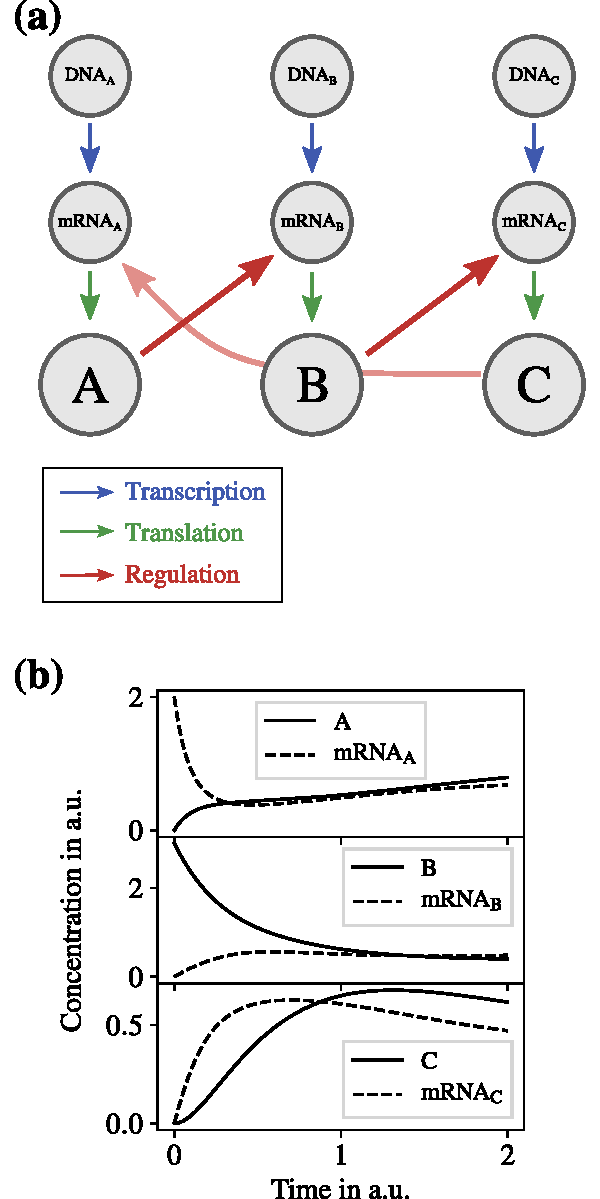
\includegraphics[width=1\columnwidth]{figures_tex/scheme}
\caption{\label{fig:network}The regulation network example described in Sec.~\ref{sec:results}.
\textbf{(a)}: Each circle depicts a species, each arrow corresponds
to one reaction. Blue arrows denote transcription from DNA to $\mathrm{mRNA}$,
green arrows denote translation from $\mathrm{mRNA}$ to protein,
and red arrows denote the regulatory network. \textbf{(b)}: Concentration
time series generated from the reaction network shown in~(a). The
initial condition prescribes positive concentration values only for
$\mathrm{B}$ protein and $\mathrm{mRNA}_{\mathrm{A}}$ species. This
initial condition is used in the subsequent sections for further analysis.}
\end{figure}

These time series of concentrations are then applied to the proposed
estimation method which is designed to find reaction networks and
rate constants from experimental data. 

\subsection{The noiseless case\label{sec:case-1}}

In this section noiseless data is generated from integrating the reaction-rate
equation (\ref{method:the-system}) of the system described in Sec.~\ref{sec:results}.
The minimization problem (\ref{method:minimizationproblem}) is solved
with respect to this data. When setting the hyperparameter $\alpha=0$
one obtains linear least-squares regression with a constraint on the
non-negativity of the estimated reaction rates.

When applying constrained linear least-squares regression, one can
observe that the sparsity pattern does not match the generating reaction
network and the reaction responsible for the decay of $\mathrm{A}$
particles is completely ignored (Fig.~\ref{fig:case-1-sparsity-pattern}).
For a suitable choice of hyperparameters $\alpha\approx1.91\cdot10^{-7}$,
$\lambda=1$, and a cutoff $\kappa=0.22$ a sparse solution can be
obtained and also the decay reaction can be recovered. The cutoff
$\kappa$ is applied so that for all reactions with an estimated rate
$\hat{\xi}<\kappa$ a rate of $\hat{\xi}=0$ is assigned. A circle
with size corresponding to a rate of $\kappa$ is depicted in Fig.~\ref{fig:case-1-sparsity-pattern}
in green.

\begin{figure}
\centering 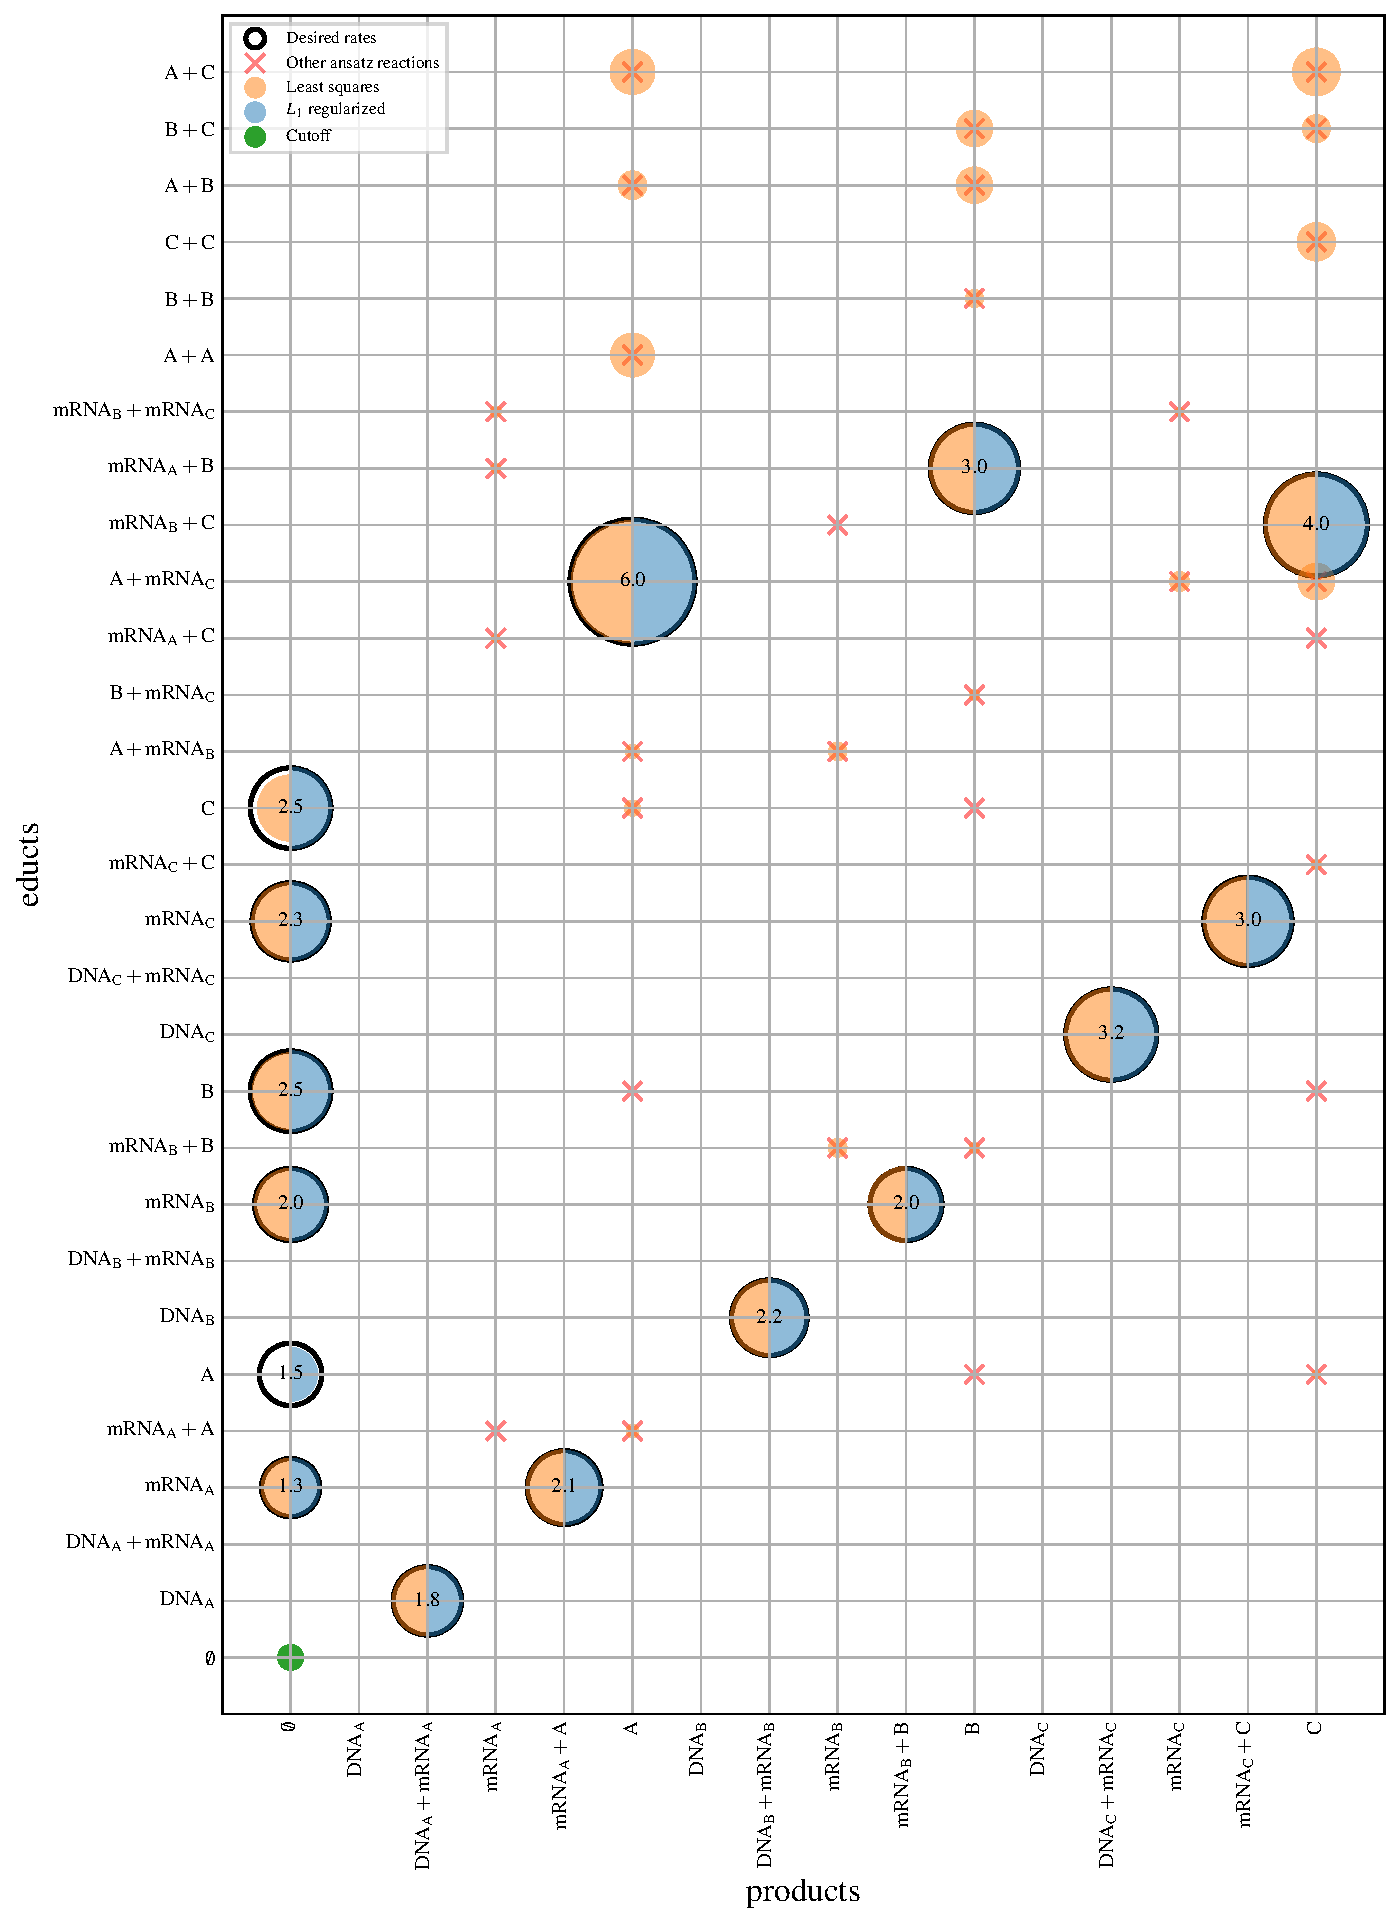
\includegraphics[width=0.9\linewidth]{figures_tex/sparsity_pattern}
\caption{\label{fig:case-1-sparsity-pattern}Estimated reaction rates in the
system described in Sec.~\ref{sec:case-1}. The y and x axes contain
reaction educts and products, respectively. A circle at position $(i,j)$
represents a reaction $i\rightharpoonup j$ whose rate has a linear
relation with the area of the circle. The black outlines denote the
reactions with which the system was generated and contain the respective
rate value. Red crosses denote reactions that were used as additional
ansatz reactions. Blue circles are estimated by linear least-squares
and orange circles depict rates which were obtained by solving the
minimization problem (\ref{method:minimizationproblem}). The latter
rates are subject to a cutoff $\kappa=0.22$ corresponding to the
green circle's area under which a sparse solution with the correct
processes can be recovered. If a certain rate was estimated in both
cases, two wedges instead of one circle are displayed.}
\end{figure}

\textbf{Todo}: 
\begin{enumerate}
\item mention finite statistics 
\item how does LSQ compensate for $A\to\emptyset$ 
\item ansatzfunctions used in $\Theta$ 
\end{enumerate}

\subsection{Data with stochastic noise\label{sec:case-2} }

For Gillespie, the initial condition contains hundreds of particles
such that the average over many realizations converges against the
reaction-rate equation.
\begin{itemize}
\item Same setup as in Section~\ref{sec:case-1} 
\item definition of failure rate 
\item $10$-fold cross validation discarding fold with test set at the (temporal)
beginning (reason: more robust hyperparameter estimation as statistical
dependence of our data is higher at the initial equilibration phase,
shuffle didn't really work well) 
\item CV was independently carried out 10 times to obtain avg/std 
\item LSQ unreliable in comparison
\item in the limit of small noise one gets a good fit 
\item obtain cutoff in noise free case -> compute failure rate (number of
false positives and negatives) 
\end{itemize}
\begin{figure}
\centering 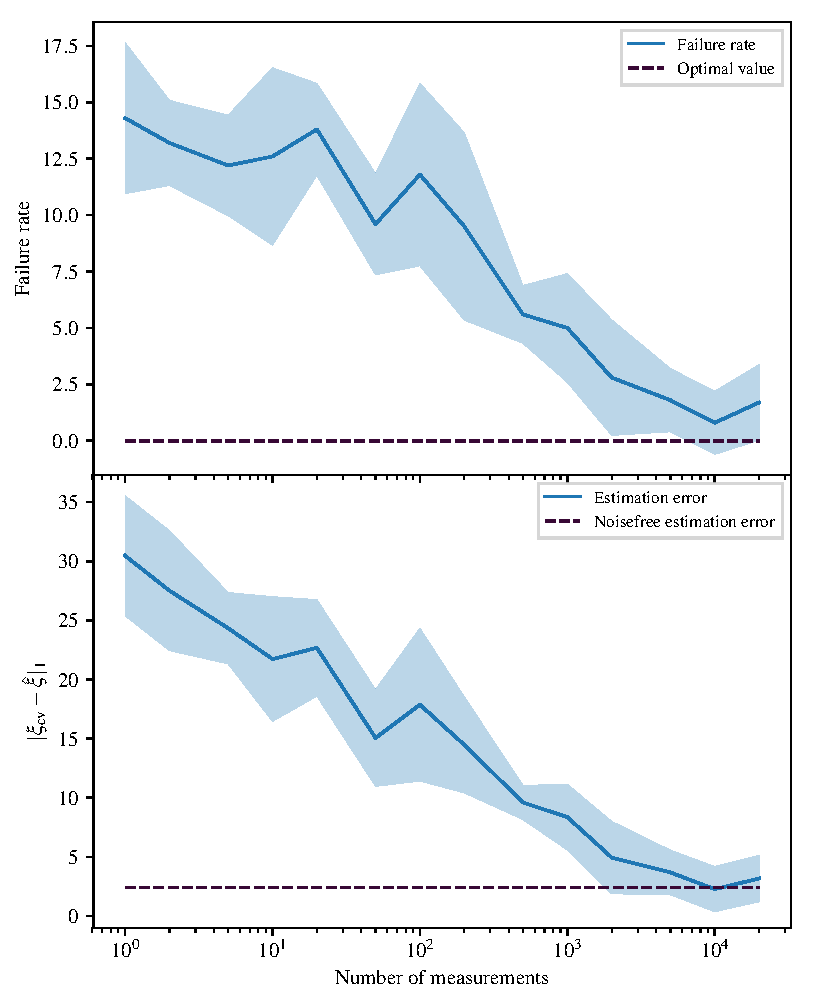
\includegraphics[width=1\columnwidth]{figures_tex/case2}
\caption{\label{fig:case2-convergence}Convergence of the estimation error
when estimating the system described in Sec.~\ref{sec:case-1} with
decreasing levels of noise by application of the minimization problem
(\ref{method:minimizationproblem}) for $\alpha=0$ (LSQ) and a $(\alpha,\lambda)$
combination found through $10$-fold cross-validation (regularized).
The level of noise is regulated by the number of measurements being
averaged. The procedure was repeated 10 times with different realizations
giving rise to the mean and standard deviation depicted by dark blue
graph and shaded blue area, respectively. The failure rate is the
number of incorrectly identified processes up to the cutoff value
introduced in Sec.~\ref{sec:case-1}. The estimation error is given
by the $L_{1}$ difference of the generating reaction rates $\xi$
and the estimated reaction rates $\hat{\xi}$.}
\end{figure}


\subsection{Multiple initial conditions\label{sec:case-3}}
\begin{itemize}
\item extend situation of Section~\ref{sec:case-3} to multiple initial
conditions (zipped / reorder) 
\item $20$-fold CV discarding 1st fold (see sec 4.2) 
\item compute failure rate 
\item model can reliably be recovered in the limit of small noise 
\end{itemize}
\begin{figure}
\centering 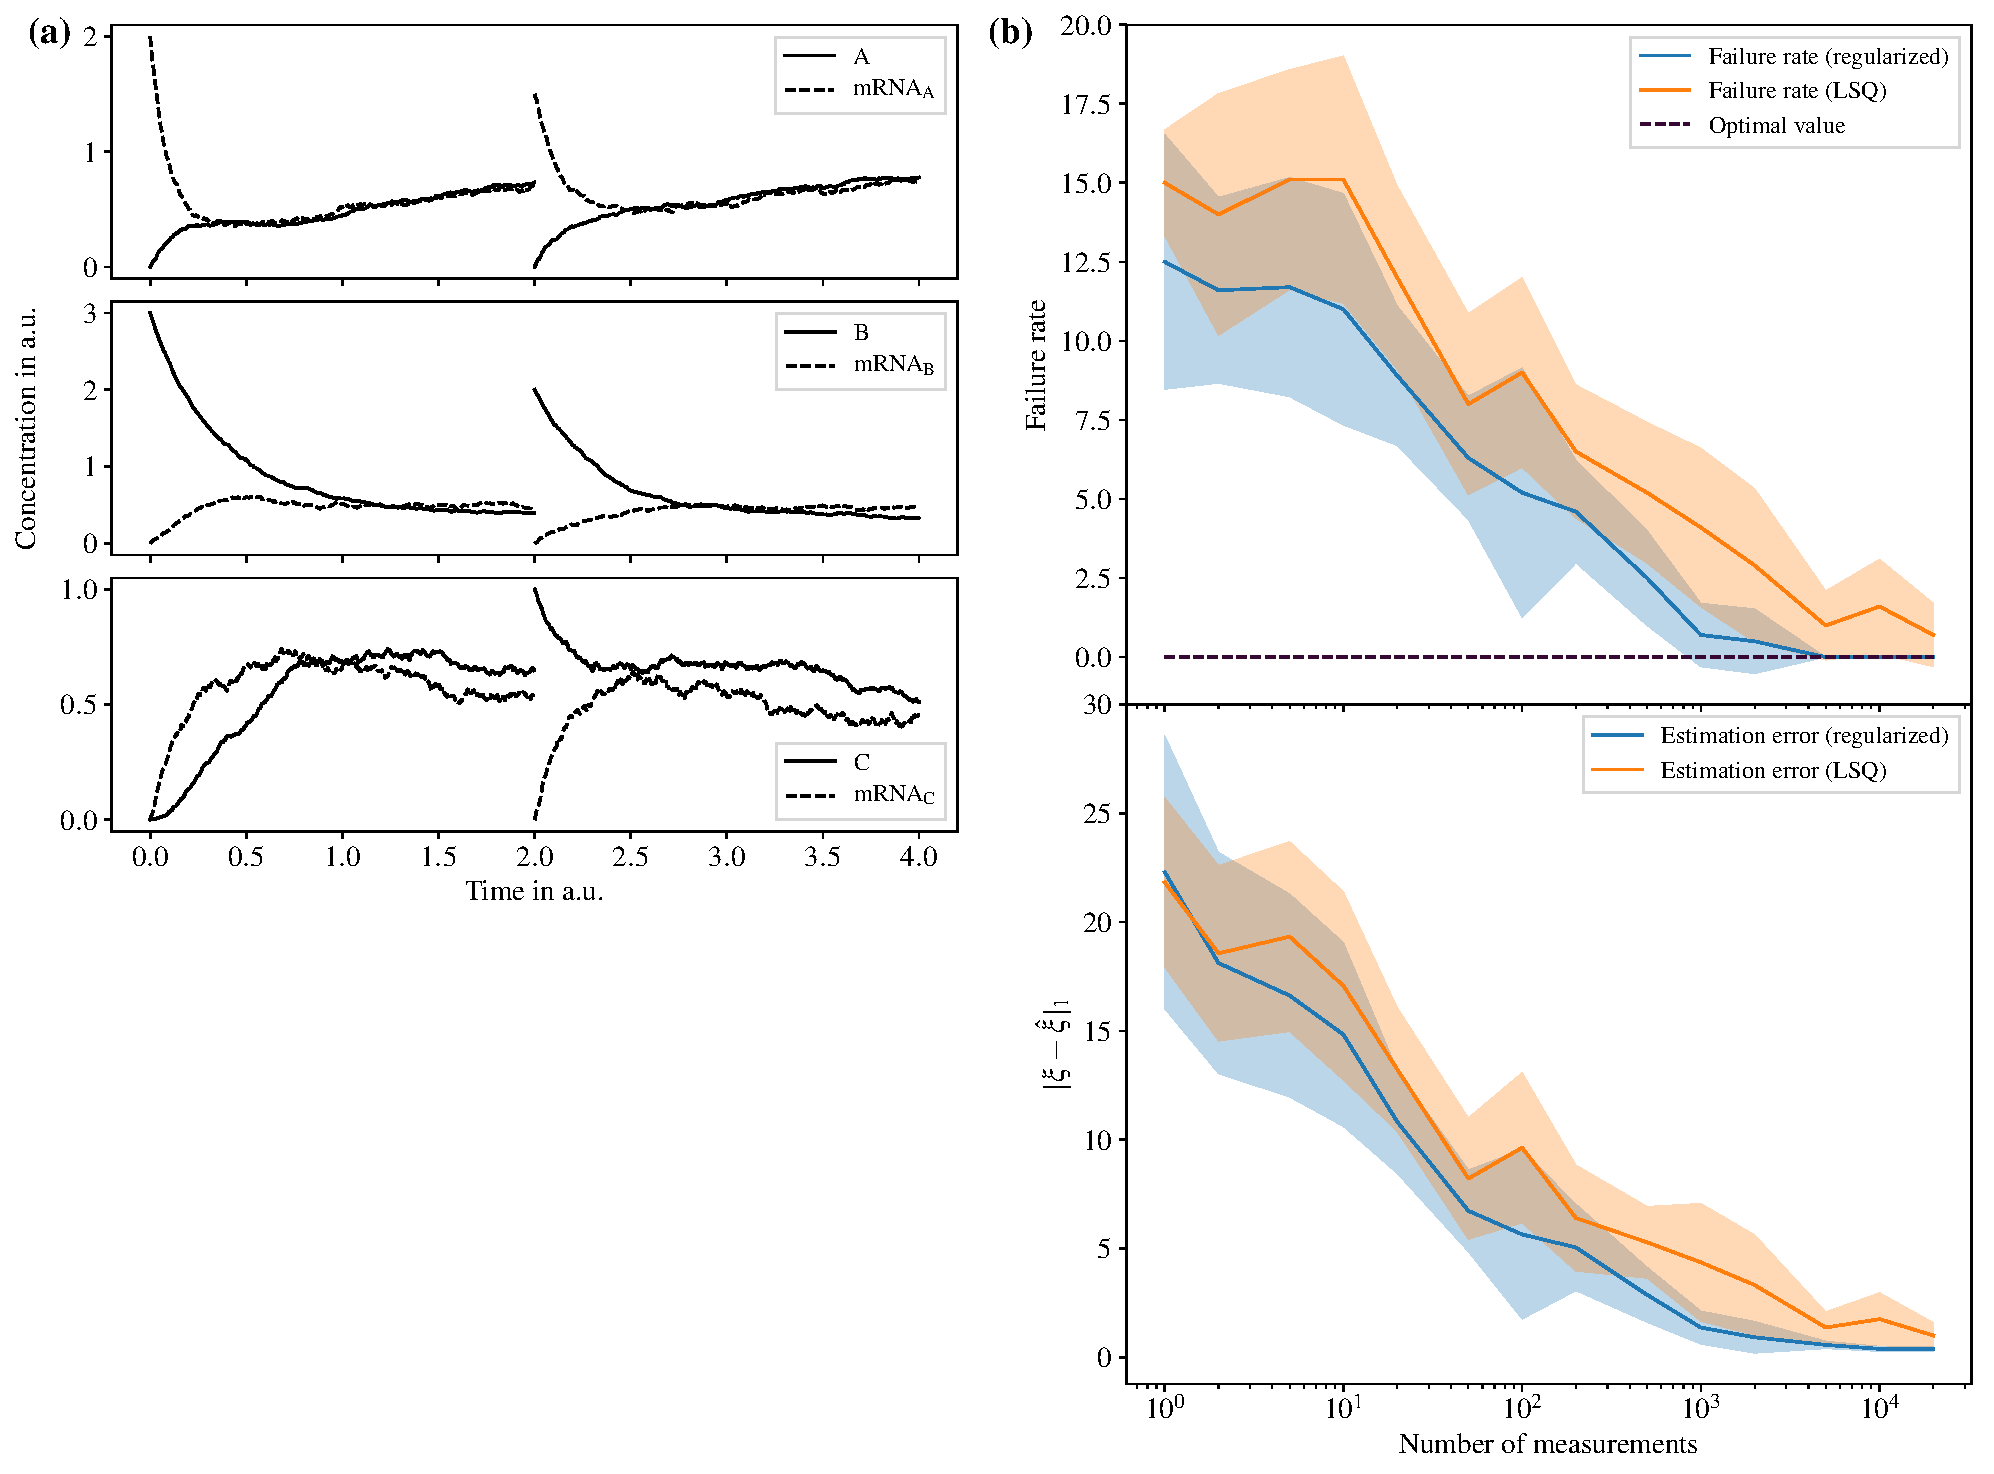
\includegraphics[width=1\columnwidth]{figures_tex/case3}
\caption{Convergence of the estimation error when using two concatenated concentration
time series with different initial conditions. \textbf{(a)}: A realization
of the concatenated timeseries. The first initial condition is identical
to what was used in Sec.~\ref{sec:case-1} and Sec.~\ref{sec:case-2}.
The second initial condition prescribes positive initial concentrations
for $\mathrm{mRNA}_{\mathrm{A}}$, $\mathrm{B}$, and $\mathrm{C}$
species. \textbf{(b)}: Analogously to Fig.~\ref{fig:case2-convergence}
with the difference that 20-fold cross validation was used for hyperparameter
estimation.}
\end{figure}


\section{Conclusion}

In this work we have successfully applied and extended the SINDy method
to not only parsimoniously detect potentially nonlinear terms in a
dynamical system from noisy data, but also yield, in this case, a
sparse set of rates with respect to generating reactions (\ref{method:the-reactions}).

%In two examples it was demonstrated that despite noisy data and unavailable derivative measurements, a parsimonious generating reaction network that is qualitatively able to explain the observed data can be estimated.
%In particular it was shown in the first example that if there is no ambiguity in the underlying model and ansatz reaction library, the actual rates can be recovered with decreasing time step, i.e., increasing resolution of the jump process.
%In the second example we could obtain an even simpler model than what was used to generate data by making use of sparse regression and cross-validation.

\newpage{} \bibliographystyle{abbrv}
\bibliography{bibliography.bib}
 \newpage{}

\section{Appendix}\label{sec:appendix}
	\begin{table}[h!]
		\centering
		\begin{tabular}{rclcc}\toprule
			\multicolumn{3}{c}{Reaction} & rate  & description \\\midrule 
			$\mathrm{DNA}_{\mathrm{A}}$  & $\rightharpoonup$ & $\mathrm{DNA}_{\mathrm{A}}+\mathrm{mRNA}_{\mathrm{A}}$  & $k_{1}=1.8$  & transcription of $\mathrm{mRNA}_{\mathrm{A}}$\\
			$\mathrm{mRNA}_{\mathrm{A}}$  & $\rightharpoonup$ & $\mathrm{mRNA}_{\mathrm{A}}+\mathrm{A}$  & $k_{2}=2.1$  & translation of $\mathrm{A}$ proteins\\
			$\mathrm{mRNA}_{\mathrm{A}}$  & $\rightharpoonup$ & $\emptyset$  & $k_{3}=1.3$  & $\mathrm{mRNA}_{\mathrm{A}}$ decay\\
			$\mathrm{A}$  & $\rightharpoonup$ & $\emptyset$  & $k_{4}=1.5$  & decay of $\mathrm{A}$ proteins\\
			$\mathrm{DNA}_{\mathrm{B}}$  & $\rightharpoonup$ & $\mathrm{DNA}_{\mathrm{B}}+\mathrm{mRNA}_{\mathrm{B}}$  & $k_{5}=2.2$  & transcription of $\mathrm{mRNA}_{\mathrm{B}}$\\
			$\mathrm{mRNA}_{\mathrm{B}}$  & $\rightharpoonup$ & $\mathrm{mRNA}_{\mathrm{B}}+\mathrm{B}$  & $k_{6}=2.0$  & translation of $\mathrm{B}$ proteins\\
			$\mathrm{mRNA}_{\mathrm{B}}$  & $\rightharpoonup$ & $\emptyset$  & $k_{7}=2.0$  & $\mathrm{mRNA}_{\mathrm{B}}$ decay\\
			$\mathrm{B}$  & $\rightharpoonup$ & $\emptyset$  & $k_{8}=2.5$  & decay of $\mathrm{B}$ proteins\\
			$\mathrm{DNA}_{\mathrm{C}}$  & $\rightharpoonup$ & $\mathrm{DNA}_{\mathrm{C}}+\mathrm{mRNA}_{\mathrm{C}}$  & $k_{9}=3.2$  & transcription of $\mathrm{mRNA}_{\mathrm{C}}$\\
			$\mathrm{mRNA}_{\mathrm{C}}$  & $\rightharpoonup$ & $\mathrm{mRNA}_{\mathrm{C}}+\mathrm{C}$  & $k_{10}=3.0$  & translation of $\mathrm{C}$ proteins\\
			$\mathrm{mRNA}_{\mathrm{C}}$  & $\rightharpoonup$ & $\emptyset$  & $k_{11}=2.3$  & $\mathrm{mRNA}_{\mathrm{C}}$ decay\\
			$\mathrm{C}$  & $\rightharpoonup$ & $\emptyset$  & $k_{12}=2.5$  & decay of $\mathrm{C}$ proteins\\
			$\mathrm{mRNA}_{\mathrm{A}}+\mathrm{A}$  & $\rightharpoonup$ & $\mathrm{A}$  & $k_{13}=0$  & self regulation of $\mathrm{A}$ proteins\\
			$\mathrm{mRNA}_{\mathrm{B}}+\mathrm{B}$  & $\rightharpoonup$ & $\mathrm{B}$  & $k_{14}=0$  & self regulation of $\mathrm{B}$ proteins\\
			$\mathrm{mRNA}_{\mathrm{C}}+\mathrm{C}$  & $\rightharpoonup$ & $\mathrm{C}$  & $k_{15}=0$  & self regulation of $\mathrm{C}$ proteins\\
			$\mathrm{mRNA}_{\mathrm{B}}+\mathrm{A}$  & $\rightharpoonup$ & $\mathrm{A}$  & $k_{16}=0$  & cyclic regulation of $\mathrm{A}$ proteins\\
			$\mathrm{mRNA}_{\mathrm{C}}+\mathrm{B}$  & $\rightharpoonup$ & $\mathrm{B}$  & $k_{17}=0$  & cyclic regulation of $\mathrm{B}$ proteins\\
			$\mathrm{mRNA}_{\mathrm{A}}+\mathrm{C}$  & $\rightharpoonup$ & $\mathrm{C}$  & $k_{18}=0$  & cyclic regulation of $\mathrm{C}$ proteins\\
			$\mathrm{mRNA}_{\mathrm{C}}+\mathrm{A}$  & $\rightharpoonup$ & $\mathrm{A}$  & $k_{16}=6.0$  & cyclic regulation of $\mathrm{A}$ proteins\\
			$\mathrm{mRNA}_{\mathrm{B}}+\mathrm{C}$  & $\rightharpoonup$ & $\mathrm{C}$  & $k_{17}=4.0$  & cyclic regulation of $\mathrm{C}$ proteins\\
			$\mathrm{mRNA}_{\mathrm{A}}+\mathrm{B}$  & $\rightharpoonup$ & $\mathrm{B}$  & $k_{18}=3.0$  & cyclic regulation of $\mathrm{B}$ proteins\\
			$\mathrm{mRNA}_{\mathrm{A}}+\mathrm{A}$  & $\rightharpoonup$ & $\mathrm{mRNA}_{\mathrm{A}}$  & $k_{19}=0$  & artificial fusion\\
			$\mathrm{mRNA}_{\mathrm{B}}+\mathrm{B}$  & $\rightharpoonup$ & $\mathrm{mRNA}_{\mathrm{B}}$  & $k_{20}=0$  & artificial fusion\\
			$\mathrm{mRNA}_{\mathrm{A}}+\mathrm{B}$  & $\rightharpoonup$ & $\mathrm{mRNA}_{\mathrm{A}}$  & $k_{21}=0$  & artificial fusion\\
			$\mathrm{mRNA}_{\mathrm{B}}+\mathrm{C}$  & $\rightharpoonup$ & $\mathrm{mRNA}_{\mathrm{B}}$  & $k_{22}=0$  & artificial fusion\\
			$\mathrm{mRNA}_{\mathrm{C}}+\mathrm{A}$  & $\rightharpoonup$ & $\mathrm{mRNA}_{\mathrm{C}}$  & $k_{23}=0$  & artificial fusion\\
			$\mathrm{mRNA}_{\mathrm{A}}+\mathrm{C}$  & $\rightharpoonup$ & $\mathrm{mRNA}_{\mathrm{A}}$  & $k_{24}=0$  & artificial fusion\\
			$\mathrm{mRNA}_{\mathrm{B}}+\mathrm{A}$  & $\rightharpoonup$ & $\mathrm{mRNA}_{\mathrm{B}}$  & $k_{25}=0$  & artificial fusion\\
			$\mathrm{A}+\mathrm{A}$  & $\rightharpoonup$ & $\mathrm{A}$  & $k_{26}=0$  & $\mathrm{A}$ regulates $\mathrm{A}$\\
			$\mathrm{B}+\mathrm{B}$  & $\rightharpoonup$ & $\mathrm{B}$  & $k_{27}=0$  & $\mathrm{B}$ regulates $\mathrm{B}$\\
			$\mathrm{C}+\mathrm{C}$  & $\rightharpoonup$ & $\mathrm{C}$  & $k_{28}=0$  & $\mathrm{C}$ regulates $\mathrm{C}$\\
			$\mathrm{B}+\mathrm{A}$  & $\rightharpoonup$ & $\mathrm{A}$  & $k_{29}=0$  & artificial fusion between proteins\\
			$\mathrm{C}+\mathrm{B}$  & $\rightharpoonup$ & $\mathrm{B}$  & $k_{30}=0$  & artificial fusion between proteins\\
			$\mathrm{A}+\mathrm{C}$  & $\rightharpoonup$ & $\mathrm{C}$  & $k_{31}=0$  & artificial fusion between proteins\\
			$\mathrm{C}+\mathrm{A}$  & $\rightharpoonup$ & $\mathrm{A}$  & $k_{32}=0$  & artificial fusion between proteins\\
			$\mathrm{B}+\mathrm{C}$  & $\rightharpoonup$ & $\mathrm{C}$  & $k_{33}=0$  & artificial fusion between proteins\\
			$\mathrm{A}+\mathrm{B}$  & $\rightharpoonup$ & $\mathrm{B}$  & $k_{34}=0$  & artificial fusion between proteins\\
			$\mathrm{A}$  & $\rightharpoonup$ & $\mathrm{B}$  & $k_{35}=0$  & artificial conversion between proteins\\
			$\mathrm{B}$  & $\rightharpoonup$ & $\mathrm{C}$  & $k_{36}=0$  & artificial conversion between proteins\\
			$\mathrm{C}$  & $\rightharpoonup$ & $\mathrm{A}$  & $k_{37}=0$  & artificial conversion between proteins\\
			$\mathrm{A}$  & $\rightharpoonup$ & $\mathrm{C}$  & $k_{38}=0$  & artificial conversion between proteins\\
			$\mathrm{C}$  & $\rightharpoonup$ & $\mathrm{B}$  & $k_{39}=0$  & artificial conversion between proteins\\
			$\mathrm{B}$  & $\rightharpoonup$ & $\mathrm{A}$  & $k_{40}=0$  & artificial conversion between proteins\\
			$\mathrm{mRNA}_{\mathrm{B}}+\mathrm{mRNA}_{\mathrm{C}}$  & $\rightharpoonup$ & $\mathrm{mRNA}_{\mathrm{A}}$  & $k_{41}=0$  & artificial fusion\\
			$\mathrm{mRNA}_{\mathrm{C}}+\mathrm{mRNA}_{\mathrm{B}}$  & $\rightharpoonup$ & $\mathrm{mRNA}_{\mathrm{C}}$  & $k_{42}=0$  & artificial fusion\\
			$\mathrm{mRNA}_{\mathrm{C}}+\mathrm{A}$  & $\rightharpoonup$ & $\mathrm{C}$  & $k_{43}=0$  & artificial fusion\\\bottomrule
		\end{tabular}\caption{\label{tab:reaction-library}Full set of ansatz reactions $\Theta$ used in Sec.~\ref{sec:results}.}
	\end{table}
\end{document}
